%%%%%%%%%%%%%%%%%%%%%%%%%%%%%%%%%%%%%%%%%
% Beamer Presentation
% LaTeX Template
% Version 1.0 (10/11/12)
%
% This template has been downloaded from:
% http://www.LaTeXTemplates.com
%
% License:
% CC BY-NC-SA 3.0 (http://creativecommons.org/licenses/by-nc-sa/3.0/)
%
%%%%%%%%%%%%%%%%%%%%%%%%%%%%%%%%%%%%%%%%%

%----------------------------------------------------------------------------------------
%	PACKAGES AND THEMES
%----------------------------------------------------------------------------------------

\documentclass[presentation]{beamer}

% The Beamer class comes with a number of default slide themes
% which change the colors and layouts of slides. Below this is a list
% of all the themes, uncomment each in turn to see what they look like.

%\usetheme{default}
%\usetheme{AnnArbor}
%\usetheme{Antibes}
%\usetheme{Bergen}
% \usetheme{Berkeley}
% \usetheme{Berlin}
%\usetheme{Boadilla}
%\usetheme{CambridgeUS}
%\usetheme{Copenhagen}
%\usetheme{Darmstadt}
% \usetheme{Dresden}
%\usetheme{Frankfurt}
%\usetheme{Goettingen}
%\usetheme{Hannover}
%\usetheme{Ilmenau}
%\usetheme{JuanLesPins}
%\usetheme{Luebeck}
\usetheme{Madrid}
%\usetheme{Malmoe}
%\usetheme{Marburg}
%\usetheme{Montpellier}
%\usetheme{PaloAlto}
%\usetheme{Pittsburgh}
%\usetheme{Rochester}
%\usetheme{Singapore}
%\usetheme{Szeged}
%\usetheme{Warsaw}

% As well as themes, the Beamer class has a number of color themes
% for any slide theme. Uncomment each of these in turn to see how it
% changes the colors of your current slide theme.

%\usecolortheme{albatross}
%\usecolortheme{beaver}
%\usecolortheme{beetle}
%\usecolortheme{crane}
%\usecolortheme{dolphin}
%\usecolortheme{dove}
%\usecolortheme{fly}
%\usecolortheme{lily}
%\usecolortheme{orchid}
%\usecolortheme{rose}
%\usecolortheme{seagull}
%\usecolortheme{seahorse}
%\usecolortheme{whale}
%\usecolortheme{wolverine}

%\setbeamertemplate{footline} % To remove the footer line in all slides uncomment this line
%\setbeamertemplate{footline}[page number] % To replace the footer line in all slides with a simple slide count uncomment this line

\setbeamertemplate{navigation symbols}{} % To remove the navigation symbols from the bottom of all slides uncomment this line

\usepackage{graphicx} % Allows including images
\usepackage{booktabs} % Allows the use of \toprule, \midrule and \bottomrule in tables
\usepackage{textpos}
\usepackage{tikz}
\usepackage{xcolor}

\newcommand\fillColor{cyan!5!white}

\title[Improved Modern Hopfield Network]{Improved Robustness and Hyperparameter Selection in the Modern Hopfield Network}
\author[School of Computing]{Hayden McAlister} 
\institute[]{
% \includegraphics[scale=0.25]{}
School of Computing, University of Otago
}
\date{Supervisors: Anthony Robins, Lech Syzmanski} 

%----------------------------------------------------------------------------------------
%	TITLE PAGE 1
%----------------------------------------------------------------------------------------
\begin{document}

\begin{frame}
\titlepage % Print the title page as the first slide
\end{frame}


%----------------------------------------------------------------------------------------
%	TITLE PAGE
%----------------------------------------------------------------------------------------

\input{slides/00_overview.tex}
% --------------------------------------------------------------------------------

\section{Introduction} 

\begin{frame}
	
\frametitle{Autoassociative Memories}

\begin{itemize}
    \item Learn to associate a state with itself.
    \item Relax probe towards a learned state.
\end{itemize}

\only<1>{
\begin{center}
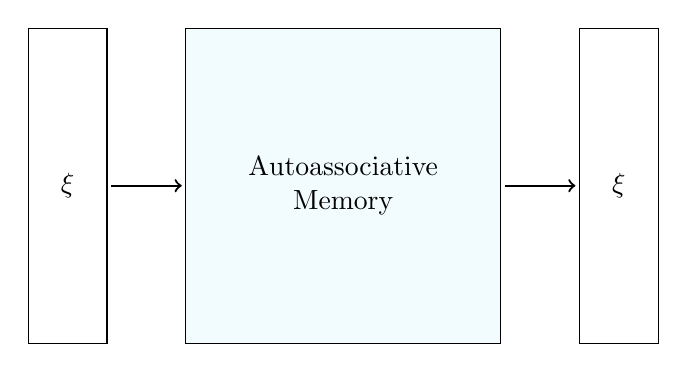
\begin{tikzpicture}
    \draw (0,0) rectangle (1,4);
    \node at (0.5,2) {$\xi$};
    \draw[thick, ->] (1.05,2) --(1.95,2);

    \filldraw[fill=\fillColor, draw=black] (2,0) rectangle (6,4);
    \node[align=center] at (4,2) {Autoassociative\\Memory};
    
    \draw (7,0) rectangle (8,4);
    \node at (7.5,2) {$\xi$};
    \draw[thick, ->] (6.05,2) --(6.95,2);
\end{tikzpicture}
\end{center}
}

\only<2>{
\begin{center}
    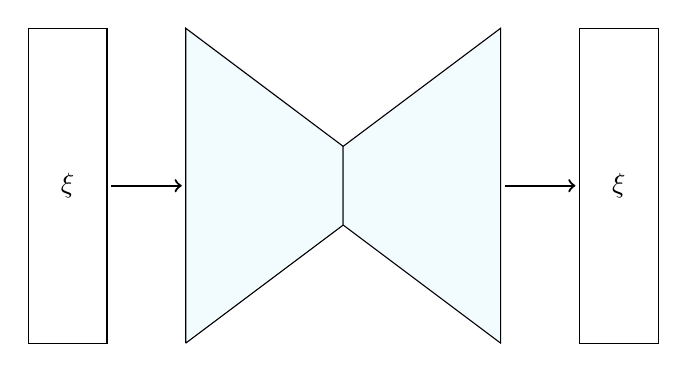
\begin{tikzpicture}
        \draw (0,0) rectangle (1,4);
        \node at (0.5,2) {$\xi$};
        \draw[thick, ->] (1.05,2) --(1.95,2);
    
        \filldraw[fill=\fillColor, draw=black] (2,0) -- (4,1.5) -- (4,2.5) --(2,4) -- (2,0);
        \filldraw[fill=\fillColor, draw=black] (4,1.5) -- (4,2.5) -- (6,4) -- (6,0) -- (4, 1.5);
        
        \draw (7,0) rectangle (8,4);
        \node at (7.5,2) {$\xi$};
        \draw[thick, ->] (6.05,2) --(6.95,2);
    \end{tikzpicture}
\end{center}
}

\only<3>{
\begin{center}
    \begin{tikzpicture}
        \draw (0,0) rectangle (1,4);
        \node at (0.5,2) {$\xi$};

        \draw[thick, ->] (1.05,2) --(6.95,2);
        
        \draw (7,0) rectangle (8,4);
        \node at (7.5,2) {$\xi$};
    \end{tikzpicture}
\end{center}
}

\only<4>{
\begin{center}
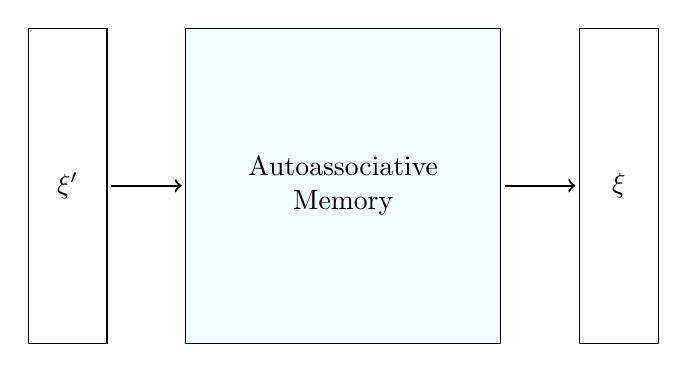
\begin{tikzpicture}
    \draw (0,0) rectangle (1,4);
    \node at (0.5,2) {$\xi^\prime$};
    \draw[thick, ->] (1.05,2) --(1.95,2);

    \filldraw[fill=\fillColor, draw=black] (2,0) rectangle (6,4);
    \node[align=center] at (4,2) {Autoassociative\\Memory};
    
    \draw (7,0) rectangle (8,4);
    \node at (7.5,2) {$\xi$};
    \draw[thick, ->] (6.05,2) --(6.95,2);
\end{tikzpicture}
\end{center}
}
    
\end{frame}

% --------------------------------------------------------------------------------

\subsection{Classical Hopfield Network} 

\begin{frame}
	
    \frametitle{Classical Hopfield Network}
    \begin{columns}[c]
        \column{.6\textwidth}
        \begin{itemize}
            \item Association by Hebbian learning.
            \begin{itemize}
                \item Biological inspiration.
                \item Easy to analyze.
            \end{itemize}
            \item Relax by matrix multiplication.
            \begin{itemize}
                \item Mean field approximation.
                \item Nonlinearity keeps states in bipolar domain.
                \item Energy guaranteed to achieve a minima (under sensible conditions).
            \end{itemize}
        \end{itemize}

        \column{.4\textwidth}
        % TODO Classical Hopfield Image
        \begin{align}
            W &= \sum_{k} \xi_k \otimes \xi_k \\
            \xi_{t+1} &= \text{ Sign}\left( W \cdot \xi_{t} \right) \\
            E \left( \xi \right) &= -\frac{1}{2} \xi^T W \xi
        \end{align}
    \end{columns}
\end{frame}

% --------------------------------------------------------------------------------

\subsection{Modern Hopfield Network} 

\begin{frame}
	
    \frametitle{Modern Hopfield Network}
    \begin{columns}[c]
        \column{.6\textwidth}
        \begin{itemize}
            \item Classical energy wells are too shallow.
            \item Key trick: Replace quadratic energy with general polynomial.
            \begin{itemize}
                \item Heck, anything with a vaguely polynomial shape.
            \end{itemize}
        \end{itemize}

        \begin{align*}
            f_n\left( x \right) &= x^n \\
            f_n\left( x \right) &= \begin{cases}
                x^n \; \text{if } x\geq0 \\
                0 \; \text{if } x<0
            \end{cases} \\
            f_n\left( x \right) &= \begin{cases}
                x^n \; \text{if } x\geq0 \\
                -\epsilon x \; \text{if } x<0
            \end{cases}
        \end{align*}

        \column{.4\textwidth}
        \only<1>{
            \begin{figure}[h]
                \includegraphics[width=\textwidth]{images/introduction_energywell01.png}
            \end{figure}
        }
        \only<2>{
            \begin{figure}[h]
                \includegraphics[width=\textwidth]{images/introduction_energywell02.png}
            \end{figure}
        }
        \only<3>{
            \begin{figure}[h]
                \includegraphics[width=\textwidth]{images/introduction_energywell03.png}
            \end{figure}
        }
        
    \end{columns}
\end{frame}

% --------------------------------------------------------------------------------

\begin{frame}
	
    \frametitle{Modern Hopfield Network}
    \begin{itemize}
        \item New hyperparameter \(n\) -- the ``interaction vertex''.
        \begin{itemize}
            \item Controls the range of influence that memories have.
            \item However, also radically alters the network architecture.
        \end{itemize}

        % TODO: Have visualizations for each of these points comparing either mathematics or visualizations with classical
        \pause
        \item Memory matrix replaced by list of memory states -- vectors of same dimension as data.
        \pause
        \item Learning no longer supports Hebbian -- now requires gradient descent.
        \pause
        \item Relaxation no longer uses mean field -- now a contrastive difference.
        \begin{itemize}
            \item Negative energy no longer means ``stable'' -- the energy \textit{difference} between a neuron clamped on and off indicates stability.
        \end{itemize}
        
    \end{itemize}
\end{frame}
% --------------------------------------------------------------------------------

\section{Behavior of the Modern Hopfield Network}

% --------------------------------------------------------------------------------

\begin{frame}
	
\frametitle{Properties -- Network Capacity}

Larger network capacities with higher interaction vertices:
\begin{align}
    K_{\text{max}} = \frac{1}{2\left(2n-3\right)!!} \frac{N^{n-1}}{\ln(N)}
\end{align}

Notably, super-linear for \(n>2\).

\end{frame}

% --------------------------------------------------------------------------------

\begin{frame}
    \frametitle{Properties -- Training Times}

Faster training times with higher interaction vertices:
\begin{figure}
    \includegraphics[width=\textwidth]{images/trainingTimes.png}
    \caption{Krotov and Hopfield 2016, Figure 01}
\end{figure}
\end{frame}

% --------------------------------------------------------------------------------

\begin{frame}
    \frametitle{Properties -- Feature to Prototype Transition}

Low interaction vertices result in memories that look like features, while higher interaction vertices result in memories that look like prototypes:

\begin{columns}
    \column{.5\textwidth}
    \begin{figure}
        \includegraphics[width=\textwidth]{images/featureDetector.png}
    \caption{Feature-like Memories, \(n=2\)}
    \end{figure}
    \column{.5\textwidth}
    \pause
    \begin{figure}
    \includegraphics[width=\textwidth]{images/randomMemories/00.png}
    \caption{Prototype-like Memories, \(n=20\)}
    \end{figure}
    % \only<1>{
    %     \begin{figure}
    %     \includegraphics[width=\textwidth]{images/randomMemories/01.png}
    %     \caption{Prototype-like Memories, \(n=20\)}
    %     \end{figure}
    % }
    % \only<2>{
    %     \begin{figure}
    %     \includegraphics[width=\textwidth]{images/randomMemories/02.png}
    %     \caption{Prototype-like Memories, \(n=20\)}
    %     \end{figure}
    % }
    % \only<3>{
    %     \begin{figure}
    %     \includegraphics[width=\textwidth]{images/randomMemories/03.png}
    %     \caption{Prototype-like Memories, \(n=20\)}
    %     \end{figure}
    % }
    
\end{columns}

\end{frame}


% \begin{frame}
%     \frametitle{Why is our implementation broken?}

%     \begin{itemize}
%         \item Other implementations online\dots
%         \begin{itemize}
%             \item Most use a feed-forward architecture that isn't as general.
%             \item An example of the autoassociative memory exists, and works!
%             \item When translated line by line to PyTorch, still broken\dots
%         \end{itemize}
%         \item Hyperparameters are numerous and ``magic''.
%     \end{itemize}
% \end{frame}
\section{Hyperparameter Search}

\begin{frame}
% \frametitle{Hyperparameter Search}
\only<1>{
    \begin{figure}
        \includegraphics[width=0.7\textwidth]{images/randomMemories/05.png}
    \caption{\(n=10\)}
    \end{figure}
}
\only<2>{
    \begin{figure}
        \includegraphics[width=0.7\textwidth]{images/randomMemories/06.png}
    \caption{\(n=15\), \(\beta=600\)}
    \end{figure}
}
\only<3>{
    \begin{figure}
        \includegraphics[width=0.7\textwidth]{images/randomMemories/07.png}
    \caption{\(n=12\), \(\beta=545\), \(\text{lr}=0.01\)}
    \end{figure}
}
\only<4>{
    \begin{figure}
        \includegraphics[width=0.7\textwidth]{images/randomMemories/08.png}
    \caption{\(n=17\), \(\beta=730\), \(\text{lr}=1.0\), \(\text{lr}_\text{decay}=0.99\)}
    \end{figure}
}
\only<5>{
    \begin{figure}
        \includegraphics[width=0.7\textwidth]{images/randomMemories/09.png}
    \caption{\(n=30\), \(\beta_i=700\), \(\beta_f=500\), \(\text{lr}=1.0\), \(\text{lr}_\text{decay}=0.99\), Interaction Function=Leaky Rectified Polynomial, \(\text{Momentum}=0.6\), \(\text{Error Power}=2\)}
    \end{figure}
}
\end{frame}

%------------------------------------------------

\begin{frame}
    \frametitle{Gridsearch of Hyperparameters}
    Let's find what (if any) hyperparameters work. Training our network on autoassociative tasks of dimension 100.
\end{frame}

%------------------------------------------------
\section{Stabilizing the Network}

% --------------------------------------------------------------------------------

% \begin{frame}
% \frametitle{Stabilizing the Network}

% \begin{itemize}
%     \item The optimal hyperparameter region shrinks as \(n\) grows.
%     \item The optimal region also shifts considerably as \(n\) grows.
%     \item When \(n\) reaches some critical threshold, the optimal region is disrupted and the network does not learn at all.
% \end{itemize}

% \end{frame}

%------------------------------------------------

\begin{frame}
    \frametitle{Network Dynamics Step by Step}
    \begin{gather*}
        \tanh \left[ \beta \sum_{\mu} \left( f_n \left(\zeta_{\mu, i} + \sum_{j \neq i} \zeta_{\mu, j} \xi_{j} \right) - f_n \left( -\zeta_{\mu, i} + \sum_{j \neq i} \zeta_{\mu, j} \xi_{j} \right) \right) \right]
    \end{gather*}

    \begin{enumerate}
        \only<1,2>{\item Calculate similarities \(\zeta \cdot \xi_{+1}, \; \zeta \cdot \xi_{-1}\)}
        \only<3->{\item \textbf{Calculate similarities \(\zeta \cdot \xi_{+1}, \; \zeta \cdot \xi_{-1}\)}}
        \only<1>{\item Pass similarities through interaction function \(f_n\)}
        \only<2->{\item \textbf{Pass similarities through interaction function \(f_n\)}}
        \item Sum the result over all memories \(\sum_\mu\)
        \item Multiply by a scaling factor \(\beta\)
        \item Pass through activation function (e.g. Sign or tanh)
    \end{enumerate}

    \only<2>{
        \begin{align*}
            f_n\left(x\right) = x^n
        \end{align*}
    }

    \only<3>{
        \begin{align*}
            \zeta, \xi \in [-1,1]^N &\implies \zeta \cdot \xi \in [-N, N] \\
        \end{align*}
    }

    \only<4>{
        \begin{align*}
            \zeta, \xi \in [-1,1]^N &\implies \zeta \cdot \xi \in [-N, N] \\
            f_n\left(\zeta \cdot \xi\right) &= \left(\zeta \cdot \xi\right)^n 
        \end{align*}
    }

    \only<5>{
        \begin{align*}
            \zeta, \xi \in [-1,1]^N &\implies \zeta \cdot \xi \in [-N, N] \\
            f_n\left(\zeta \cdot \xi\right) &= \left(\zeta \cdot \xi\right)^n \\
                &= N^n
        \end{align*}
    }

\end{frame}

\begin{frame}
    \frametitle{How large is too large?}

    \begin{center}
        \begin{tabular}{| c | c |}
            \hline
            Network parameters & Interaction function value \\
            \hline
            \hline
            \(N=100, n=2\) & \(10^{4}\) \\
            \hline
            \(N=100, n=5\) & \(10^{10}\) \\
            \hline
            \(N=100, n=10\) & \(10^{18.89}\) \\
            \hline
            \(N=100, n=20\) & \(10^{40}\) \\
            \hline
        \end{tabular}
    \end{center}

    \pause
    Maximum value of a float32 is \(\approx 3.4 \cdot 10^{38}\). Default data type of PyTorch.

    \pause
    Maximum value of a float64 is \(\approx 1.8 \cdot 10^{304}\). Default data type of numpy.
\end{frame}

\begin{frame}
    \frametitle{Stabilizing the Network}
    
    \begin{itemize}
        \item The optimal hyperparameter region shrinks as \(n\) grows.
        \pause
        \item The optimal region also shifts considerably as \(n\) grows.
        \pause
        \item When \(n\) reaches some critical threshold, the optimal region is disrupted and the network does not learn at all.
        \pause
        \begin{itemize}
            \item This is because the memories are learned to be prototypes for large \(n\), which have large similarities scores with the probe states, and are made larger by the interaction function.
        \end{itemize}
    \end{itemize}    
\end{frame}
    

\begin{frame}
    \frametitle{Fixing the Problem}
    \only<1>{
        \begin{gather*}
            \tanh \left[ \beta \sum_{\mu} \left( f_n \left(\zeta_{\mu, i} + \sum_{j \neq i} \zeta_{\mu, j} \xi_{j} \right) - f_n \left( -\zeta_{\mu, i} + \sum_{j \neq i} \zeta_{\mu, j} \xi_{j} \right) \right) \right]
        \end{gather*}
    }
    \only<2>{
        \begin{gather*}
            \tanh \left[ \textcolor{red}{\boldsymbol \beta} \sum_{\mu} \left( f_n \left(\zeta_{\mu, i} + \sum_{j \neq i} \zeta_{\mu, j} \xi_{j} \right) - f_n \left( -\zeta_{\mu, i} + \sum_{j \neq i} \zeta_{\mu, j} \xi_{j} \right) \right) \right]
        \end{gather*}
    }
    \only<3>{
        \begin{gather*}
            \tanh \left[ \sum_{\mu} \left( \textcolor{red}{\boldsymbol \beta} f_n \left(\zeta_{\mu, i} + \sum_{j \neq i} \zeta_{\mu, j} \xi_{j} \right) - \textcolor{red}{\boldsymbol \beta} f_n \left( -\zeta_{\mu, i} + \sum_{j \neq i} \zeta_{\mu, j} \xi_{j} \right) \right) \right]
        \end{gather*}
    }
    \only<4>{
        \begin{gather*}
            \tanh \left[ \sum_{\mu} \left( f_n \left(\textcolor{red}{\boldsymbol \beta} \left(\zeta_{\mu, i} + \sum_{j \neq i} \zeta_{\mu, j} \xi_{j} \right) \right) - f_n \left(\textcolor{red}{\boldsymbol \beta} \left( -\zeta_{\mu, i} + \sum_{j \neq i} \zeta_{\mu, j} \xi_{j} \right) \right) \right) \right]
        \end{gather*}
        \begin{center}
            If \(f_n\) is homogenous: \(f(\alpha x) = \alpha^k f(x)\). \\
            Weaker than linear -- includes Polynomial and Rectified Polynomial.
        \end{center}
    }

    \only<5>{
        \begin{gather*}
            \tanh \left[ \sum_{\mu} \left( f_n \left(\textcolor{red}{\frac{\boldsymbol \beta}{N}} \left(\zeta_{\mu, i} + \sum_{j \neq i} \zeta_{\mu, j} \xi_{j} \right) \right) - f_n \left(\textcolor{red}{\frac{\boldsymbol \beta}{N}} \left( -\zeta_{\mu, i} + \sum_{j \neq i} \zeta_{\mu, j} \xi_{j} \right) \right) \right) \right]
        \end{gather*}
        \begin{center}
            If \(f_n\) is homogenous: \(f(\alpha x) = \alpha^k f(x)\). \\
            Weaker than linear -- includes Polynomial and Rectified Polynomial.
        \end{center}
    }
\end{frame}

% \input{slides/05_components_and_tools_used}
% \input{slides/06_implementation}
% 
\section{Final Results and Prototype}

\begin{frame}
\frametitle{Final Results and Prototype}
\begin{theorem}[Mass--energy equivalence]
$E = mc^2$
\end{theorem}
\end{frame}

%------------------------------------------------


\begin{frame}[fragile] % Need to use the fragile option when verbatim is used in the slide
\frametitle{Verbatim}
\begin{example}[Theorem Slide Code]
\begin{verbatim}
\begin{frame}
\frametitle{Theorem}
\begin{theorem}[Mass--energy equivalence]
$E = mc^2$
\end{theorem}
\end{frame}\end{verbatim}
\end{example}
\end{frame}

%------------------------------------------------
% 
\section{Work plan and task allocation}
\begin{frame}
\frametitle{Work plan and task allocation}
Uncomment the code on this slide to include your own image from the same directory as the template .TeX file.
%\begin{figure}
%\includegraphics[width=0.8\linewidth]{test}
%\end{figure}
\end{frame}

%------------------------------------------------
% 
\section{Conclusion}
\begin{frame}[fragile] % Need to use the fragile option when verbatim is used in the slide
\frametitle{Conclusion}
An example of the \verb|\cite| command to cite within the presentation:\\~

This statement requires citation.
\end{frame}

%------------------------------------------------
% \section{References}

\begin{frame}
\frametitle{References}
% \footnotesize{
% \begin{thebibliography}{99} % Beamer does not support BibTeX so references must be inserted manually as below
% \end{thebibliography}
% }
\end{frame}

%------------------------------------------------

%----------------------------------------------------------------------------------------


\end{document} 